\documentclass{article}

\usepackage{graphicx}
\usepackage{tikz}
\usepackage{tikzsymbols}
\usetikzlibrary{calc,patterns,shapes.geometric}
\pagestyle{empty}
\usepackage[margin=0pt]{geometry}
\geometry{papersize={14in,12in}}

\def\centerarc[#1](#2)(#3:#4:#5){\draw[#1] ($(#2)+({#5*cos(#3)},{#5*sin(#3)})$) arc (#3:#4:#5);}

\begin{document}
	\begin{figure}
		\centering
		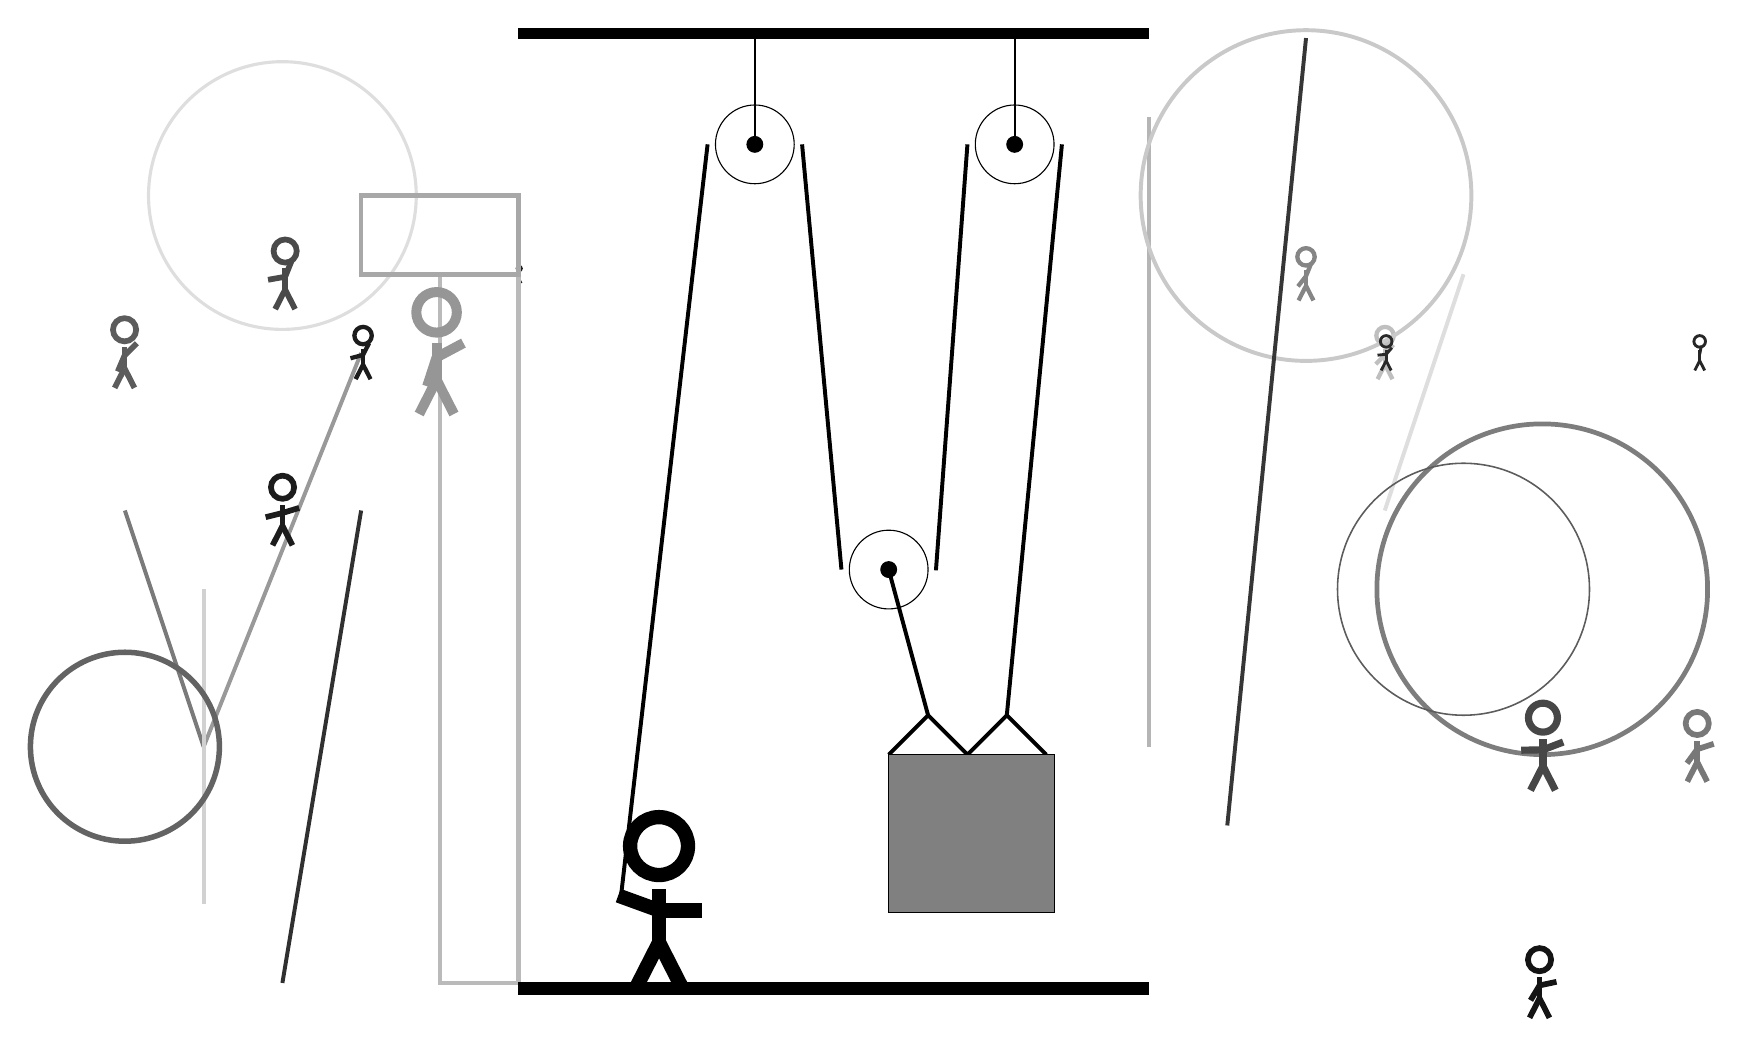
\begin{tikzpicture}
			%%%%% START %%%%%
			
			\draw[fill=black] (-2, 9) rectangle (6, 9.125);
			
			\draw[line width=0.5mm, color=black!29](6, 8) -- (6, 0);
			
			\node[line width=0.6mm, color=black!25] at (9, 5) {\Strichmaxerl[3][45][51]};
			\node[line width=0.5mm, color=black!88] at (-2, 6) {\Strichmaxerl[1][19][85]};
			\draw[line width=0.5mm, color=black!81](-4, 3) -- (-5, -3);
			\draw[line width=0.5mm, color=black!52](-7, 3) -- (-6, 0);
			\draw [line width=0.5mm, color=black!21](8, 7) circle (2.1);
			
			\draw[line width=0.5mm, color=black!40](-4, 5) -- (-6, 0);
			\draw[line width=0.5mm, color=black!79](7, -1) -- (8, 9);
			\draw [line width=0.4mm, color=black!13](-5, 7) circle (1.7);
			
			\draw[line width=0.5mm, color=black!18](-6, -2) -- (-6, 2);
			
			\node[line width=0.5mm, color=black!53] at (13, 0) {\Strichmaxerl[4][54][18]};
			
			\draw[line width=0.5mm, color=black!13](10, 6) -- (9, 3);
			\draw [line width=0.6mm, color=black!51](11, 2) circle (2.1);
			\node[line width=0.4mm, color=black!89] at (-5, 3) {\Strichmaxerl[4][14][17]};
			\draw[line width=0.6mm, color=black!27] (-2, -3) rectangle (-3, 6);
			\node[line width=0.4mm, color=black!64] at (-7, 5) {\Strichmaxerl[4][67][45]};
			
			\node[line width=0.6mm, color=black!48] at (8, 6) {\Strichmaxerl[3][52][68]};
			
			\node[line width=0.5mm, color=black!92] at (11, -3) {\Strichmaxerl[4][59][12]};
			\node[line width=0.7mm, color=black!71] at (-5, 6) {\Strichmaxerl[4][10][68]};
			\node[line width=0.4mm, color=black!89] at (-4, 5) {\Strichmaxerl[3][15][63]};
			\node[line width=0.2mm, color=black!85] at (13, 5) {\Strichmaxerl[2][90][79]};
			
			\draw [line width=0.2mm, color=black!64](10, 2) circle (1.6);
			
			\draw[line width=0.6mm, color=black!34] (-4, 7) rectangle (-2, 6);
			\node[line width=0.7mm, color=black!41] at (-3, 5) {\Strichmaxerl[7][72][28]};
			\node[line width=0.4mm, color=black!72] at (11, 0) {\Strichmaxerl[5][1][21]};
			
			\node[line width=0.7mm, color=black!84] at (9, 5) {\Strichmaxerl[2][6][49]};
			
			\draw [line width=0.7mm, color=black!61](-7, 0) circle (1.2);
			
			\draw (1, 7.65) circle (0.5);
			\draw[fill=black] (1, 7.65) circle (0.1);
			\draw[thick] (1, 7.65) -- (1, 9);
			
			\draw (4.3, 7.65) circle (0.5);
			\draw[fill=black] (4.3, 7.65) circle (0.1);
			\draw[thick] (4.3, 7.65) -- (4.3, 9);
			
			\draw (2.7, 2.25) circle (0.5);
			\draw[fill=black] (2.7, 2.25) circle (0.1);
			
			\draw[line width=0.5mm]  (2.7, -0.1) -- (3.2, 0.4) -- (3.7, -0.1) -- (4.2, 0.4) -- (4.7, -0.1);
			\draw[fill=black!50] (2.7, -0.1) rectangle (4.8, -2.1);
			
			\draw[line width=0.5mm](-0.7, -1.9) -- (0.4, 7.65);
			\centerarc[line width=0.5mm](1, 7.65)(0:180:0.6);
			\draw[line width=0.5mm](1.6, 7.65) -- (2.1, 2.25);
			\centerarc[line width=0.5mm](2.7, 2.25)(180:370:0.6);
			\draw[line width=0.5mm] (3.3, 2.24) -- (3.7, 7.65);
			\centerarc[line width=0.5mm](4.3, 7.65)(0:180:0.6);
			\draw[line width=0.5mm](4.2, 0.4) -- (4.9, 7.65);
			\draw[line width=0.5mm] (3.2, 0.4) -- (2.7, 2.25);
			
			\node at (-0.2, -2) {\Strichmaxerl[10][-20][0]};
			
			\draw[fill=black] (-2, -3) rectangle (6, -3.15);
			
			%%%%% END %%%%%
		\end{tikzpicture}
	\end{figure}	
\end{document}